\chapter{Materiales y métodos}

\section{Diseño metodológico del proyecto}
En el proyecto se empleó el modelo de desarrollo incremental de \textit{software}, el cual permite dividir los esfuerzos en incrementos, 
de forma que cada uno se integra con los anteriores y se prueba de manera independiente. Se optó por seguir esta metodología
puesto que en las primeras etapas se desconocía las tecnologías empleadas más allá de sus fundamentos, por lo que se requería de 
un proceso de aprendizaje y experimentación que permitiera la familiarización con las herramientas a emplear a la par que se 
concretaba el diseño final y los requisitos principales que se debían cubrir.

\section{Entorno de trabajo}
Durante el desarrollo del proyecto se empleó un entorno de trabajo basado en linux, específicamente la 
distribución \textit{Linux Mint 22.2} con el entorno de escritorio \textit{Cinnamon}. 
Se empleó un equipo con las siguientes características:
\begin{itemize}
    \item Procesador: AMD Ryzen 7 3700X.
    \item Memoria RAM: 16 GB DDR4.
    \item Almacenamiento: 500 GB SSD NVMe 2.0. 2TB HDD.
    \item Tarjeta gráfica: NVIDIA GeForce RTX 3070.
\end{itemize}

En lo referente a los dispositivos móviles empleados para la prueba de la aplicación, se emplearon los siguientes:
\begin{itemize}
    \item \textbf{Xiaomi 11T Pro} con sistema operativo Android 14
    \item \textbf{iPhone 15 Plus:} con sistema operativo iOS 26
\end{itemize}

Debido a la carencia de equipamiento específico, no se emplearon robots físicos, sino que fueron simulados mediante el uso de un \textit{software}, 
concretamente \textit{Gazebo}, que permite la simulación de robots y entornos en 3D.

Para el desarrollo \textit{software} se emplearon las siguientes herramientas:
\begin{itemize}
    \item \textbf{Visual Studio Code:} IDE para el desarrollo de aplicaciones web y de escritorio, que incluye herramientas de depuración y extensiones para diferentes lenguajes de programación.
    \item \textbf{Git:} Sistema de control de versiones distribuido, que
    permite llevar un registro de los cambios realizados en el código fuente y colaborar con otros desarrolladores.
    \item \textbf{GitHub:} Plataforma de alojamiento de repositorios Git, que permite compartir el código fuente y colaborar con otros desarrolladores.
    \item \textbf{Unity:} Motor de desarrollo de videojuegos y aplicaciones interactivas, que permite crear aplicaciones para diferentes plataformas, incluyendo Android.
    \item \textbf{Android Studio:} IDE para el desarrollo de aplicaciones Android, que incluye herramientas de depuración y emulación de dispositivos. 
    En concreto, se empleó para las pruebas de contenerización del servicio ROS necesario para el funcionamiento de la aplicación, puesto que permite 
    la instalación de \textit{termux} y la consiguiente ejecución de contenedores en un entorno Android. 
    \item \textbf{Unity Hub:} Herramienta de gestión de proyectos y versiones de Unity, que permite crear y administrar proyectos de Unity y descargar diferentes versiones del motor.
    \item \textbf{ROS:} Sistema operativo para robots, que proporciona un conjunto de herramientas y bibliotecas para el desarrollo de aplicaciones robóticas.
    \item \textbf{C\#:} Lenguaje de programación orientado a objetos, que se empleó para el desarrollo de la aplicación en Unity.
    \item \textbf{Python:} Lenguaje de programación interpretado, que se empleó para el desarrollo de los nodos ROS.
    \item \textbf{C++:} Lenguaje de programación compilado, que se empleó para el desarrollo del plugin de detección de AprilTags.
    \item \textbf{Termux:} Emulador de terminal para Android, que permite ejecutar aplicaciones de línea de comandos y contenedores en un entorno Android.
    \item \textbf{Gazebo:} Simulador de robots y entornos en 3D, que permite la simulación de robots y entornos en un entorno virtual.
    \item \textbf{Rviz:} Herramienta de visualización de datos de ROS, que permite visualizar los datos generados por los nodos ROS en un entorno gráfico.
    \item \textbf{Terminator:} Emulador de terminal para Linux, que permite ejecutar aplicaciones de línea de comandos en un entorno Linux.
    \item \textbf{Terminal de Linux:} Emulador de terminal para Linux, que permite ejecutar aplicaciones de línea de comandos en un entorno Linux.
    \item \textbf{Draw.io:} Herramienta web que permite crear diagramas UML, de entidad relación, flujogramas, etc.
\end{itemize}

\section{Materiales empleados}
Para la realización del proyecto se emplearon los siguientes materiales y repositorios:
\begin{itemize}
    \item \textbf{ROS-TCP-Endpoint:} Paquete de ROS que permite la comunicación entre un nodo ROS y una aplicación externa a través de TCP/IP.
    \item \textbf{ROS-TCP-Connector:} Interfaz C\# de alto nivel para la comunicación entre la aplicación y los nodos ROS.
    \item \textbf{AprilTags:} Sistema de marcadores visuales que permite la detección y seguimiento de objetos en imágenes y videos.
    \item \textbf{AprilRobotics/apriltag:} Librería C++ que permite la detección y seguimiento de los marcadores visuales (\textit{AprilTags}).
\end{itemize}

\section{Análisis de requisitos}
A continuación se muestran los requisitos funcionales y no funcionales que deben ser cubiertos en el proyecto.

\subsection{Requisitos funcionales}
\begin{longtable}{|p{2cm}|p{4cm}|p{7cm}|p{2cm}|}
\hline
\textbf{ID} & \textbf{Nombre} & \textbf{Descripción} & \textbf{Prioridad} \\
\hline
RF-001 & Conexión con ROS & El sistema permitirá se contectará al servidor TCP-IP para realizar solicitudes. & Alta \\
\hline
RF-002 & Detección de marcas visuales & El sistema deberá reconocer marcas visuales características (\textit{AprilTags}).  & Alta \\
\hline
RF-003 & Asignación de \textit{frames} a marcas visuales & El usuario podrá asignar un \textit{frame} concreto a una marca visual (\textit{AprilTags}).  & Alta \\
\hline
RF-004 & Visualización \textit{frames} & El sistema permitirá a los usuarios visualizar los \textit{frames} presentes en el sistema. & Alta \\
\hline
RF-005 & Visualización orientación \textit{frames} & El sistema permitirá conocer la orientación de los \textit{frames} en todo momento.  & Alta \\
\hline
RF-006 & Visualización posición \textit{frames} & El sistema permitirá conocer la posición de los \textit{frames} en todo momento.  & Alta \\
\hline
RF-007 & Visualización estado \textit{frames} & El sistema permitirá conocer el estado de los \textit{frames} (activo, parado o \textit{idle}). & Alta \\
\hline
RF-008 & Visualización velocidad lineal \textit{frames} & El sistema permitirá conocer la velocidad lineal de los \textit{frames}. & Alta \\
\hline
RF-009 & Visualización velocidad angular \textit{frames} & El sistema permitirá conocer la velocidad angular de los \textit{frames}. & Alta \\
\hline
RF-010 & Visualización \textit{jitter} \textit{frames} & El sistema permitirá conocer si el \textit{frame} tiene \textit{jitter} (fluctuación en tiempo ejecución de instrucciones). & Media \\
\hline
RF-011 & Visualización \textit{jump} \textit{frames} & El sistema permitirá conocer si el \textit{frame} se mueve con saltos (\textit{jump}). & Media \\
\hline
RF-012 & Visualización \textit{flipping} \textit{frames} & El sistema permitirá conocer si el \textit{frame} se produce \textit{flipping}. & Media \\
\hline
RF-013 & Ocultar visualización \textit{frames} & El sistema permitirá ocultar \textit{frames}. & Alta \\
\hline
RF-014 & Ajuste posición \textit{frames} asignados & El sistema permitirá ajustar la posición de los \textit{frames} asignados a los \textit{AprilTag}. & Media \\
\hline
RF-015 & Ajuste escala \textit{frames} & El sistema permitirá ajustar la escala de los \textit{frames}. & Media \\
\hline
RF-016 & Medición \textit{frames} & El sistema permitirá conocer la distancia que existe entre dos \textit{frames}. & Baja \\
\hline
RF-017 & Configuración \textit{frames} nube puntos & El usuario podrá asociar a cada \textit{frame} un \textit{topic} en el que se emitan mensajes PointCloud2 (nube de puntos). & Baja \\
\hline
RF-018 & Visualización nubes de puntos \textit{frames} & El sistema mostrará las nubes de puntos de sensores en los \textit{frames} configurados. & Baja \\
\hline
RF-019 & Parar ejecución & El sistema permitirá pausar momentáneamente la actualización de la posición de los \textit{frames} para que puedan realizarse comprobaciones. & Baja \\
\hline
RF-020 & Configuración del \textit{frame} objetivo de ruta planificada & El usuario podrá asignar el \textit{topic} encargado de la publicación de la ruta planificada al \textit{frame} raíz. & Media \\
\hline
RF-021 & Visualización de ruta planificada & El sistema permitirá conocer la ruta planificada de cada \textit{frame}. & Media \\
\hline
RF-022 & Planificación de ruta & El sistema permitirá crear un plan de ruta para un robot concreto (empleando \textit{topic} específico). & Media \\
\hline
RF-023 & Operación remota (teleoperación) & El sistema permitirá operar a cada robot de forma independiente (empleando \textit{topic} específico). & Media \\
\hline
RF-024 & Suscripción a \textit{topics} & El usuario podrá suscribirse a \textit{topics} y observar los contenidos publicados en ellos. & Baja \\
\hline
RF-025 & Publicación en \textit{topics} & El usuario podrá publicar mensajes en \textit{topics} específicos. & Baja \\
\hline
RF-026 & Modificación de parámetros & El usuario podrá modificar parámetros de los nodos. & Baja \\
\hline
RF-027 & Configuración de ajustes & El usuario podrá modificar los ajustes de conexión, del sistema de reconocimiento de marcas visuales, lenguaje, etc. & Alta \\
\hline
\end{longtable}

\subsection{Requisitos no funcionales}
\begin{longtable}{|p{2cm}|p{3.5cm}|p{7.5cm}|p{2cm}|}
\hline
\textbf{ID} & \textbf{Categoría} & \textbf{Descripción} & \textbf{Prioridad} \\
\hline
RNF-001 & Usbilidad & Deben evitrarse las interacciones innecesarias del usuario priorizando la configuración automática cuando sea posible para reducir carga cognitiva.  & Alta \\
\hline
RNF-002 & Escalabilidad & Los módulos deben desarrollarse teniendo en cuenta la posibilidad de su ampliación y la inclusión futura de sistemas de \textit{plugins}.  & Alta \\
\hline
\end{longtable}

\subsection{Casos de uso}
\subsubsection{CU-01: Configuración conexión ROS}

\textbf{Actor Principal:} Usuario

\textbf{Objetivo:}
Establecer exitosamente la conexión con ROS.

\textbf{Precondiciones:}
\begin{itemize}
    \item El servidor auxiliar de la aplicación debe estar ejecutandose dentro de la misma red o en otra.
    \item Conocer la dirección IP del servidor.
    \item Conocer el puerto en el que se expone el servicio. 
\end{itemize}

\textbf{Flujo Principal:}
\begin{enumerate}
    \item El usuario accede a la configuración.
    \item El usuario introduce la dirección IP.
    \item El usuario introduce el puerto.
    \item El usuario modifica otros parámetros como el tiempo de vida de conexión, la conexión en el inicio, etc.
    \item El usuario guarda los cambios.
    \item El sistema almacena la informacion y restablece la conexión con los nuevos parámetros.
    \item Se visualizan los \textit{frames} presentes en el grafo ROS.
\end{enumerate}

\textbf{Flujos Alternativos:}
\begin{itemize}
    \item Dirección IP o puerto no válido: El sistema no muestra los \textit{frames}.
\end{itemize}

\subsubsection{CU-02: Configuración idioma}

\textbf{Actor Principal:} Usuario

\textbf{Objetivo:}
Establecer exitosamente el idioma.

\textbf{Precondiciones:}
-

\textbf{Flujo Principal:}
\begin{enumerate}
    \item El usuario accede a la configuración.
    \item El usuario selecciona el idioma deseado.
    \item El usuario guarda los cambios.
    \item El sistema modifica los textos de la aplicación.
\end{enumerate}

\textbf{Flujos Alternativos:}
-

\subsubsection{CU-03: Asignación de \textit{frame} a \textit{AprilTag}}

\textbf{Actor Principal:} Usuario

\textbf{Objetivo:}
Asociar exitosamente un \textit{AprilTag} a un \textit{frame}.

\textbf{Precondiciones:}
\begin{itemize}
    \item El servidor auxiliar de la aplicación debe estar ejecutandose dentro de la misma red o en otra.
    \item La conexión debe haberse establecido de forma exitosa.
    \item El \textit{AprilTag} debe no haber sido asociado anteriormente o liberado de su asignación.
\end{itemize}

\textbf{Flujo Principal:}
\begin{enumerate}
    \item El usuario enfoca la camara del dispositivo hacia un \textit{AprilTag}.
    \item El sistema detecta el \textit{AprilTag} y determina si ha sido asignado.
    \item Si no ha sido asignado (o se ha liberado), se solicita al usuario que asocie la marca visual a un \textit{frame} concreto.
    \item El usuario selecciona el \textit{frame} y guarda los cambios.
    \item El sistema almacena la asiganción.
\end{enumerate}

\textbf{Flujos Alternativos:}
\begin{itemize}
    \item Si la marca visual ya está asignada no se solicitará al usuario la validación.
\end{itemize}

\subsubsection{CU-04: Configuración nube de puntos}

\textbf{Actor Principal:} Usuario

\textbf{Objetivo:}
Establecer exitosamente la configuración de los nube de puntos para los \textit{frames}.

\textbf{Precondiciones:}
\begin{itemize}
    \item El servidor auxiliar de la aplicación debe estar ejecutandose dentro de la misma red o en otra.
    \item La conexión debe haberse establecido de forma exitosa.
\end{itemize}

\textbf{Flujo Principal:}
\begin{enumerate}
    \item El usuario accede a la configuración.
    \item El usuario selecciona un \textit{frame}.
    \item El usuario selecciona el \textit{topic} al que corresponde la nube de puntos.
    \item El sistema almacena la informacion.
    \item Se visualiza la nube de puntos en los \textit{frames} correspondientes.
\end{enumerate}

\textbf{Flujos Alternativos:}
-

\subsubsection{CU-05: Configuración visualización ruta planificada}

\textbf{Actor Principal:} Usuario

\textbf{Objetivo:}
Establecer exitosamente la visualización de la ruta planificada.

\textbf{Precondiciones:}
\begin{itemize}
    \item El servidor auxiliar de la aplicación debe estar ejecutandose dentro de la misma red o en otra.
    \item La conexión debe haberse establecido de forma exitosa.
\end{itemize}

\textbf{Flujo Principal:}
\begin{enumerate}
    \item El usuario enfoca la camara del dispositivo hacia un \textit{AprilTag}.
    \item El sistema detecta el \textit{AprilTag} y determina si ha sido asignado.
    \item Si no ha sido asignado (o se ha liberado), se solicita al usuario que asocie la marca visual a un \textit{frame} concreto.
    \item El usuario selecciona el \textit{topic} de la visualización de ruta planificada y guarda los cambios.
    \item El sistema almacena la asiganción.
\end{enumerate}

\textbf{Flujos Alternativos:}
\begin{itemize}
    \item Si la marca visual ya está asignada no se solicitará al usuario la validación.
\end{itemize}

\subsubsection{CU-06: Visualizar/Ocultar \textit{frames}}

\textbf{Actor Principal:} Usuario

\textbf{Objetivo:}
Realizar exitosamente la ocultación/visualización de un \textit{frame}.

\textbf{Precondiciones:}
\begin{itemize}
    \item El servidor auxiliar de la aplicación debe estar ejecutandose dentro de la misma red o en otra. 
    \item La conexión debe haberse establecido de forma exitosa.
\end{itemize}

\textbf{Flujo Principal:}
\begin{enumerate}
    \item El usuario accede a la configuración.
    \item El usuario selecciona el \textit{frame} objetivo.
    \item El usuario activa/desactiva el \textit{frame}.
    \item El sistema visualiza/oculta el \textit{frame} seleccionado.
\end{enumerate}

\textbf{Flujos Alternativos:}
-

\subsubsection{CU-07: Teleoperación}

\textbf{Actor Principal:} Usuario

\textbf{Objetivo:}
Realizar exitosamente la operación telemática de un robot.

\textbf{Precondiciones:}
\begin{itemize}
    \item El servidor auxiliar de la aplicación debe estar ejecutandose dentro de la misma red o en otra. 
    \item La conexión debe haberse establecido de forma exitosa.
\end{itemize}

\textbf{Flujo Principal:}
\begin{enumerate}
    \item El usuario accede a la teleoperación.
    \item El usuario selecciona el \textit{topic} objetivo del movimiento.
    \item El usuario acciona los controles virtuales.
    \item El sistema envia el mensaje al \textit{topic} seleccionado.
    \item El robot se mueve correspondiendo a las ordenes realizadas.
\end{enumerate}

\textbf{Flujos Alternativos:}
-

\subsubsection{CU-08: Planificar ruta}

\textbf{Actor Principal:} Usuario

\textbf{Objetivo:}
Realizar exitosamente la planificación de la ruta de un robot.

\textbf{Precondiciones:}
\begin{itemize}
    \item El servidor auxiliar de la aplicación debe estar ejecutandose dentro de la misma red o en otra. 
    \item La conexión debe haberse establecido de forma exitosa.
\end{itemize}

\textbf{Flujo Principal:}
\begin{enumerate}
    \item El usuario accede a la planificación de ruta.
    \item El usuario selecciona el \textit{topic} objetivo de la planificación.
    \item El usuario añade/elimina puntos objetivos para el robot.
    \item El usuario ejecuta la ruta.
    \item El sistema envia punto a punto la ruta al \textit{topic} objetivo.
\end{enumerate}

\textbf{Flujos Alternativos:}
-

\subsubsection{CU-09: Medición entre \textit{frames}}

\textbf{Actor Principal:} Usuario

\textbf{Objetivo:}
Realizar exitosamente la medición de la distancia entre \textit{frames}.

\textbf{Precondiciones:}
\begin{itemize}
    \item El servidor auxiliar de la aplicación debe estar ejecutandose dentro de la misma red o en otra. 
    \item La conexión debe haberse establecido de forma exitosa.
\end{itemize}

\textbf{Flujo Principal:}
\begin{enumerate}
    \item El usuario accede a la medición.
    \item El usuario selecciona un \textit{frame} de los presentes.
    \item El usuario selecciona otro \textit{frame}.
    \item El sistema calcula la distancia, la rotación, etc.
\end{enumerate}

\textbf{Flujos Alternativos:}
-

\subsubsection{CU-10: Ajuste de posición de \textit{frames} asignados a marcas visuales}

\textbf{Actor Principal:} Usuario

\textbf{Objetivo:}
Realizar exitosamente el ajuste de la posición de \textit{frames} en las marcas visuales.

\textbf{Precondiciones:}
\begin{itemize}
    \item El servidor auxiliar de la aplicación debe estar ejecutandose dentro de la misma red o en otra. 
    \item La conexión debe haberse establecido de forma exitosa.
\end{itemize}

\textbf{Flujo Principal:}
\begin{enumerate}
    \item El usuario accede al ajuste de \textit{frames}.  
    \item El usuario ajusta un \textit{frame} raiz.
    \item El sistema almacena el ajuste y lo aplica constantemente.
\end{enumerate}

\textbf{Flujos Alternativos:}
-

\subsubsection{CU-11: Ajuste de escala de \textit{frames} asignados a marcas visuales}

\textbf{Actor Principal:} Usuario

\textbf{Objetivo:}
Realizar exitosamente el ajuste de la escala de un \textit{frame}.

\textbf{Precondiciones:}
\begin{itemize}
    \item El servidor auxiliar de la aplicación debe estar ejecutandose dentro de la misma red o en otra. 
    \item La conexión debe haberse establecido de forma exitosa.
\end{itemize}

\textbf{Flujo Principal:}
\begin{enumerate}
    \item El usuario accede al ajuste de \textit{frames}.  
    \item El usuario selecciona un \textit{frame}.
    \item El usuario aumenta o disminuye la escala de un frame.
    \item El sistema almacena el ajuste y lo aplica constantemente.
\end{enumerate}

\textbf{Flujos Alternativos:}
-

\subsubsection{CU-12: Suscripción a \textit{topics}}

\textbf{Actor Principal:} Usuario

\textbf{Objetivo:}
Realizar exitosamente la suscripción a un \textit{topic}.

\textbf{Precondiciones:}
\begin{itemize}
    \item El servidor auxiliar de la aplicación debe estar ejecutandose dentro de la misma red o en otra. 
    \item La conexión debe haberse establecido de forma exitosa.
\end{itemize}

\textbf{Flujo Principal:}
\begin{enumerate}
    \item El usuario accede a la suscripción.  
    \item El usuario selecciona un \textit{topic}.
    \item El usuario verifica la selección.
    \item El sistema se suscribe al \textit{topic} y muestra los mensajes al usuario.
\end{enumerate}

\textbf{Flujos Alternativos:}
-

\subsubsection{CU-13: Publicación en \textit{topics}}

\textbf{Actor Principal:} Usuario

\textbf{Objetivo:}
Realizar exitosamente la pulblicación de un mensaje en un \textit{topic}.

\textbf{Precondiciones:}
\begin{itemize}
    \item El servidor auxiliar de la aplicación debe estar ejecutandose dentro de la misma red o en otra. 
    \item La conexión debe haberse establecido de forma exitosa.
\end{itemize}

\textbf{Flujo Principal:}
\begin{enumerate}
    \item El usuario accede a la publicación.  
    \item El usuario selecciona un \textit{topic}.
    \item El usuario selecciona un tipo de mensaje.
    \item El usuario introduce el mensaje.
    \item El usuario introduce selecciona la frecuencia de publicación.
    \item El usuario verifica la selección.
    \item El sistema se publica el mensaje al \textit{topic} seleccionado.
\end{enumerate}

\textbf{Flujos Alternativos:}
-

\subsubsection{CU-14: Modificación de parámetros en nodos}

\textbf{Actor Principal:} Usuario

\textbf{Objetivo:}
Realizar exitosamente la modificación de un parámetro en un nodo.

\textbf{Precondiciones:}
\begin{itemize}
    \item El servidor auxiliar de la aplicación debe estar ejecutandose dentro de la misma red o en otra. 
    \item La conexión debe haberse establecido de forma exitosa.
\end{itemize}

\textbf{Flujo Principal:}
\begin{enumerate}
    \item El usuario accede a la modificación de parámetros.  
    \item El usuario selecciona un parámetro.
    \item El usuario introduce el nuevo del valor del parámetro.
    \item El sistema envía el valor del parámetro al nodo.
\end{enumerate}

\textbf{Flujos Alternativos:}
-


\section{Diseño del sistema}
En este apartado se muestran los diagramas de los módulos principales de la aplicación,
los cuales se describen en el apartado de implementación del sistema.

En la Figura \ref{fig:tf_module} se muestra el diagrama del módulo 
de transformaciones de ROS, el cual se encarga de reconstruir la jerarquía 
de ROS en Unity y mostrarla al usuario mediante diferentes funcionalidades (visualización de velocidades,
saltos, \textit{trail}, etc.).
\begin{figure}[htbp]
    \centering
    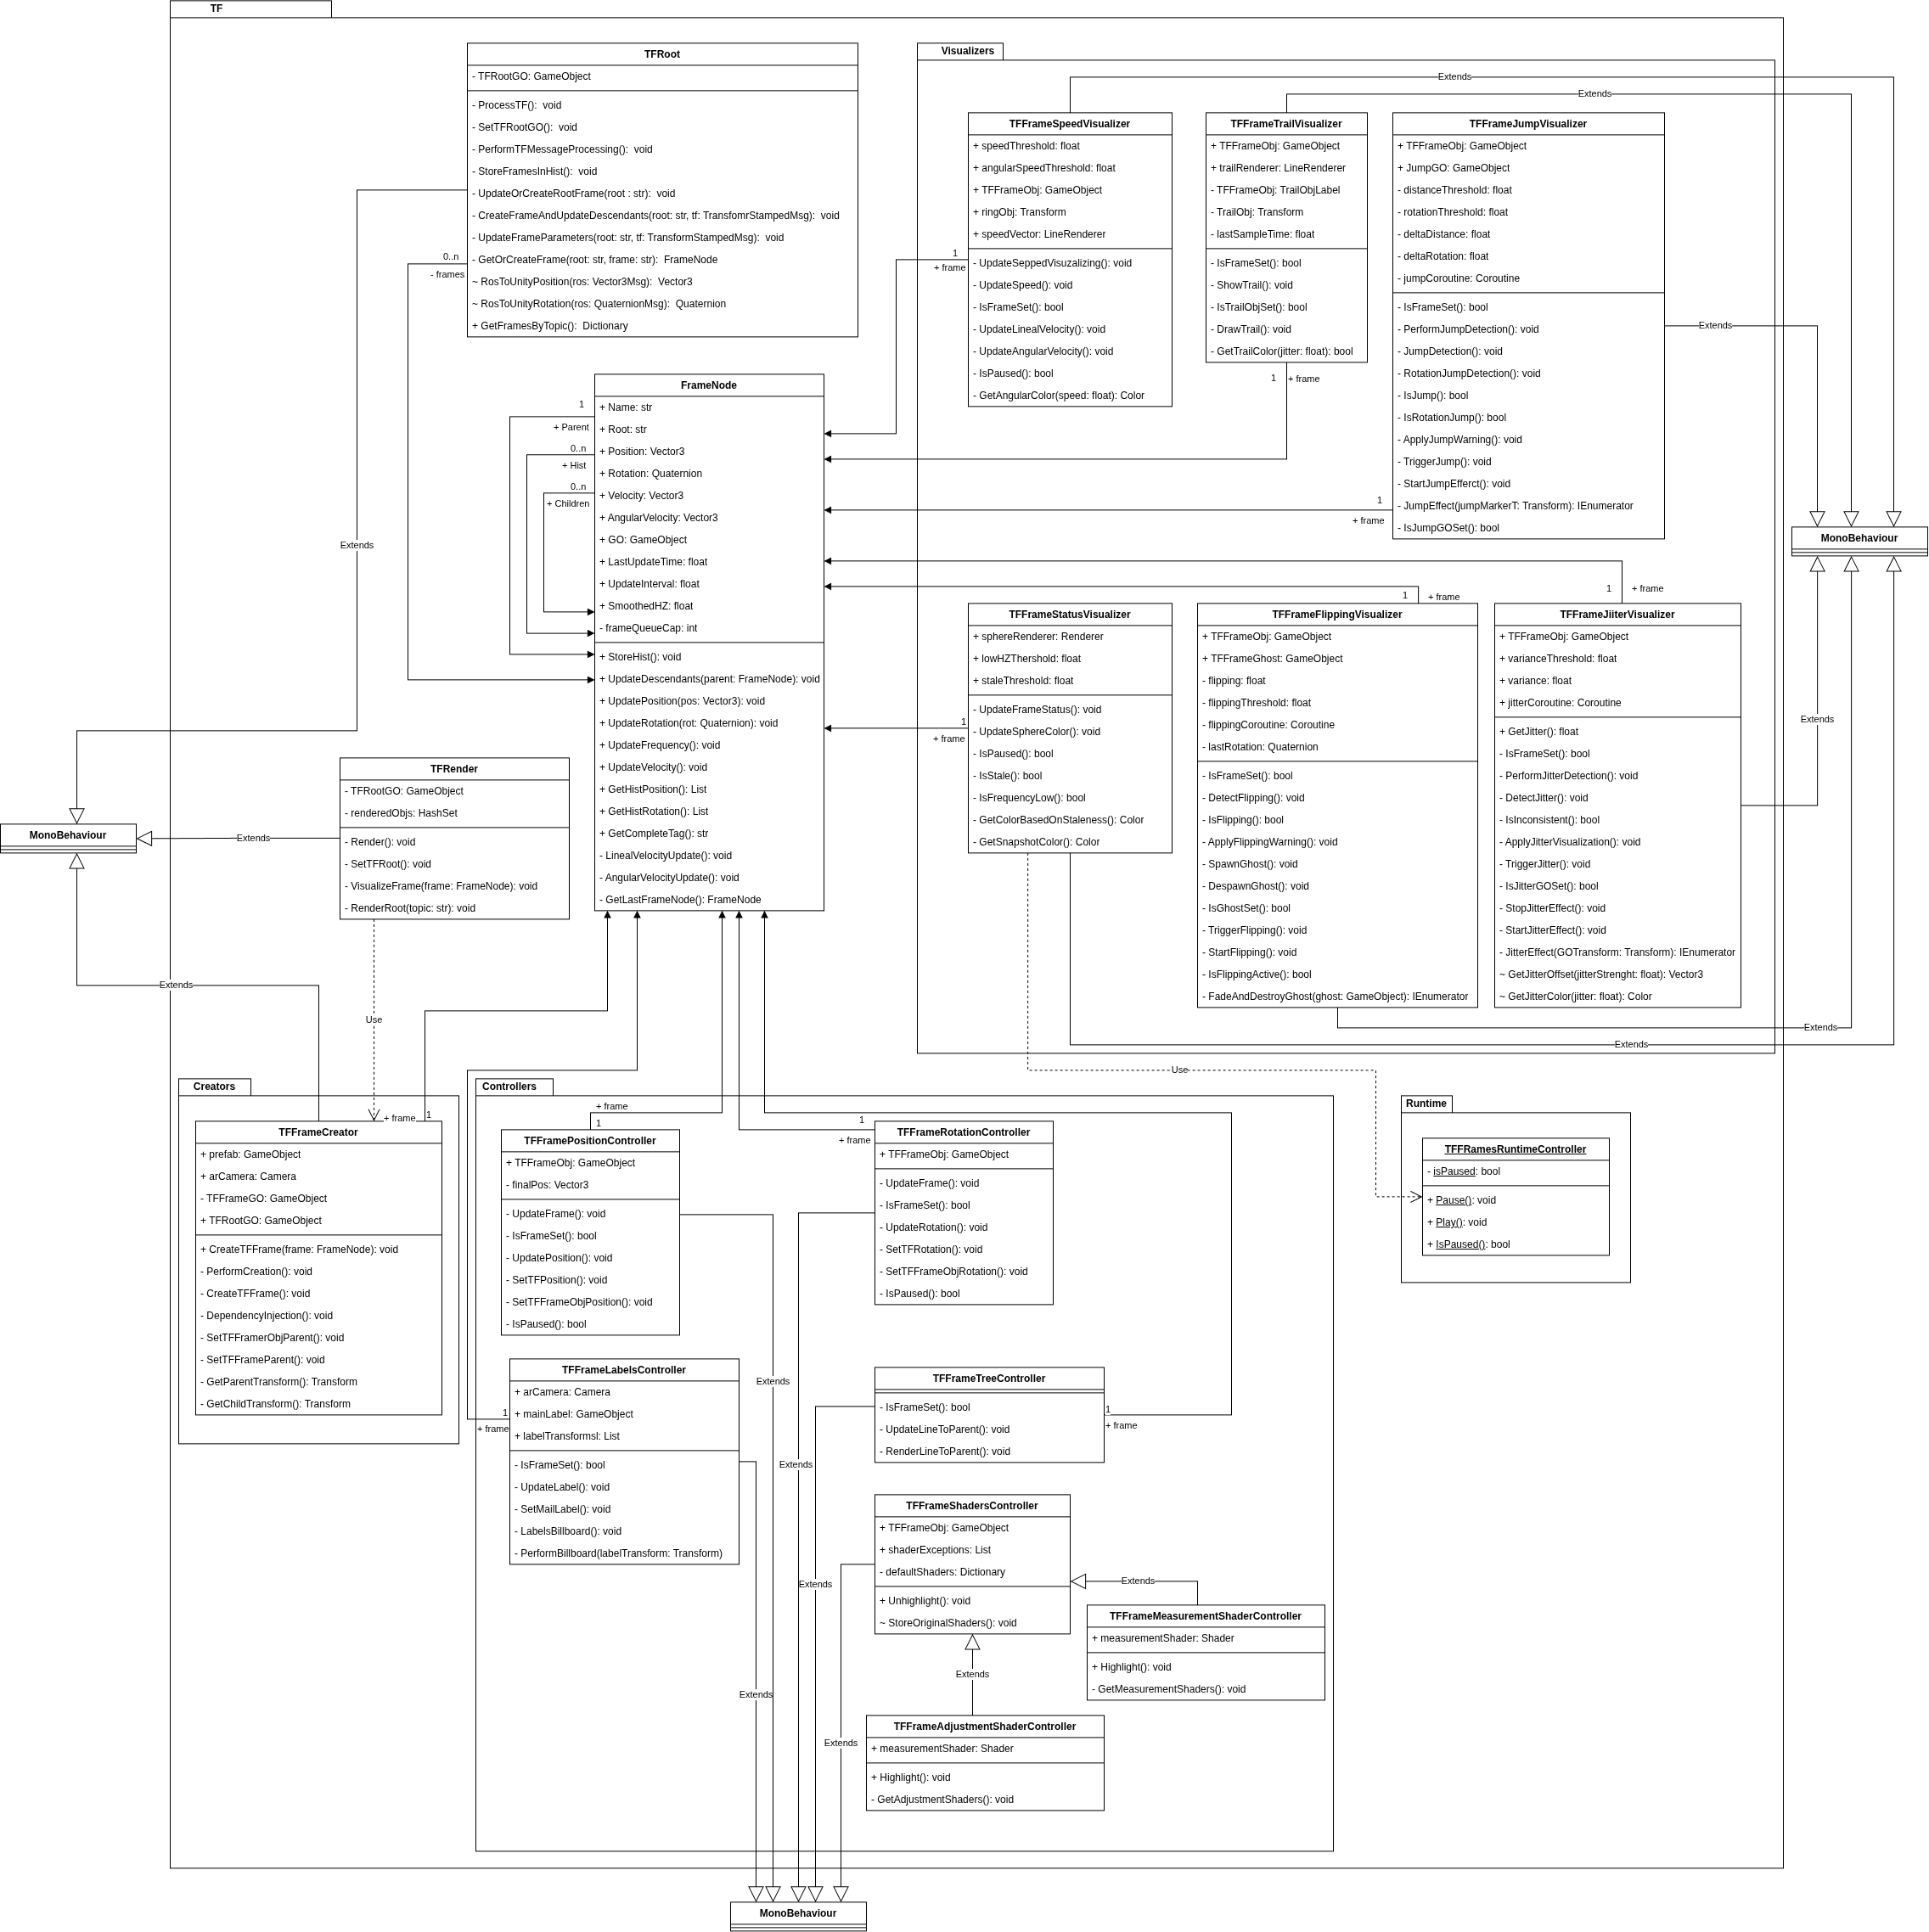
\includegraphics[width=0.8\textwidth]{imagenes/diagramas/TF.png}
    \caption{Módulo TF}
    \label{fig:tf_module}
\end{figure}

La Figura \ref{fig:point_clouds_module} muestra el diagrama del módulo de nubes de puntos, 
el cual se encarga de mostrar en el mundo virtual las nubes de puntos emitidas por los sensores de detección de profundidad como \textit{LiDAR}.
\begin{figure}[htbp]
    \centering
    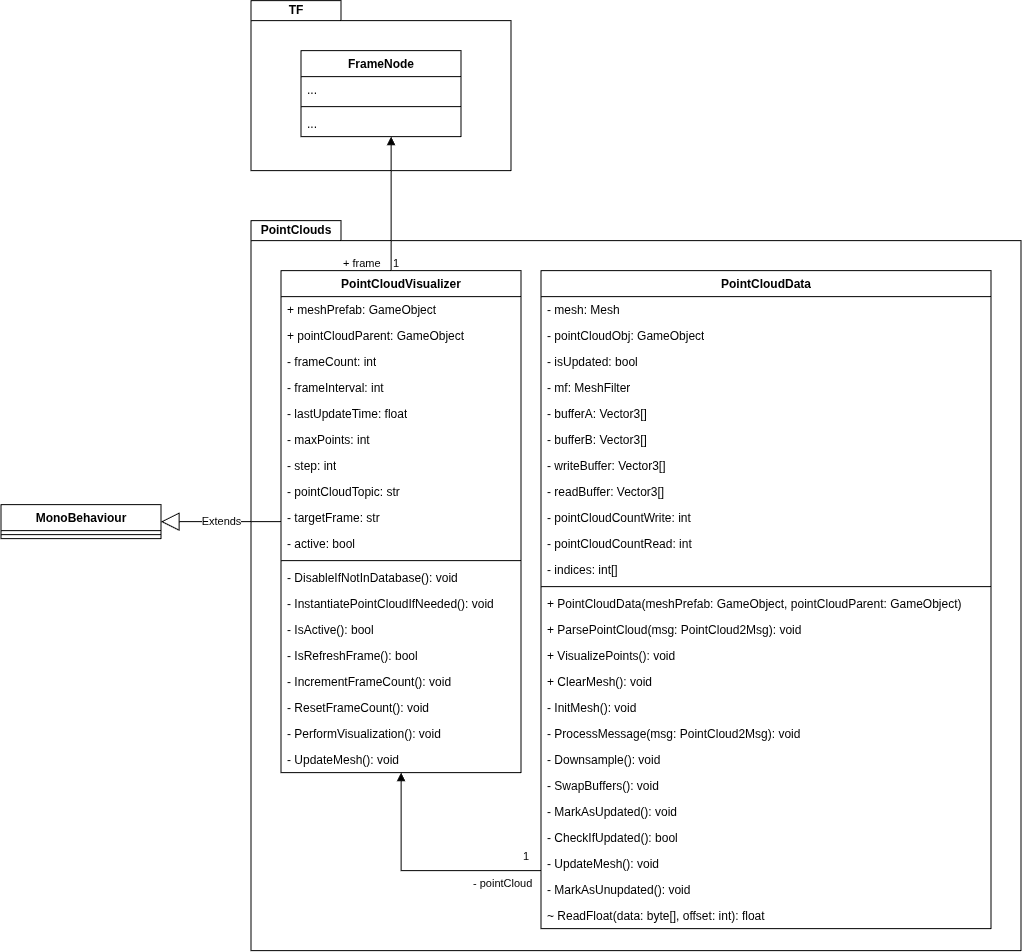
\includegraphics[width=0.8\textwidth]{imagenes/diagramas/PointClouds.png}
    \caption{Módulo PointClouds}
    \label{fig:point_clouds_module}
\end{figure}

En la Figura \ref{fig:spatial_control_module} se muestra el diagrama del módulo de control espacial.
Este se encarga de permitir la planificación de rutas y visualizarlas en el mundo virtual.
\begin{figure}[htbp]
    \centering
    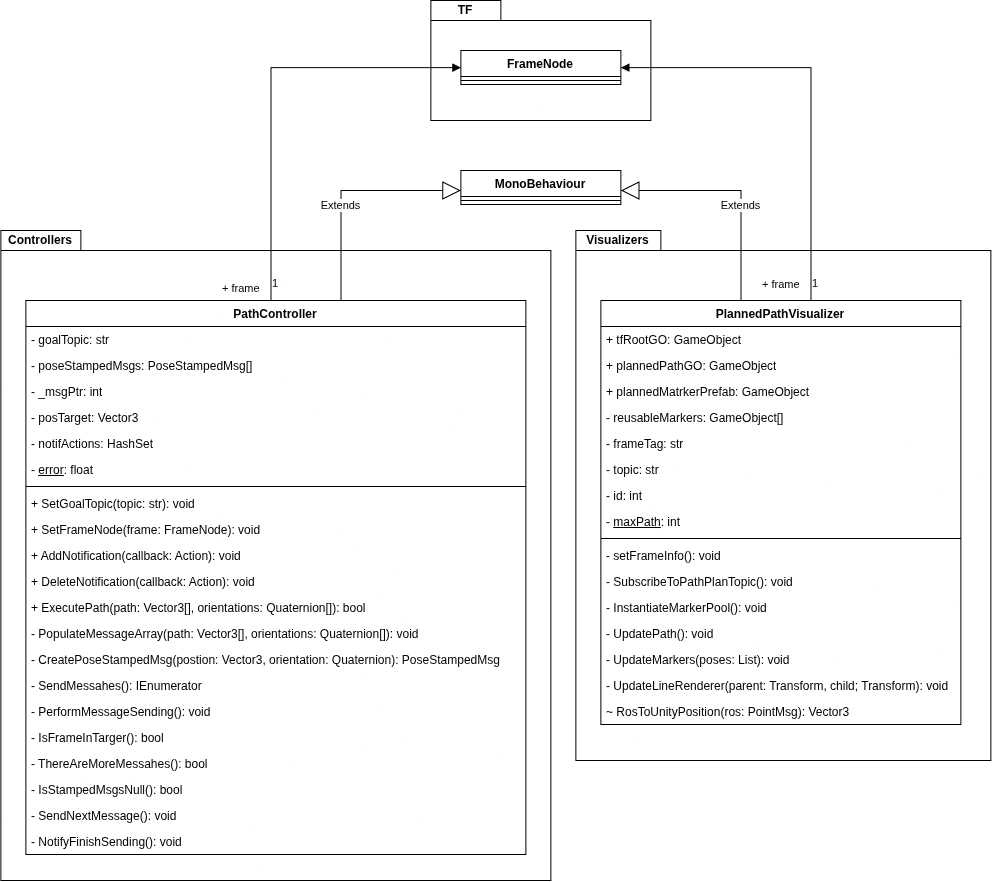
\includegraphics[width=0.8\textwidth]{imagenes/diagramas/SpatialControl.png}
    \caption{Módulo SpatialControl}
    \label{fig:spatial_control_module}
\end{figure}

El módulo de suscripción a temas de ROS se muestra en la Figura \ref{fig:ros_subscriber_module}.
Este se encarga de establecer la comunicación con los nodos de ROS y recibir los mensajes 
publicados en los \textit{topics} a los que se suscribe, para ello, se emplea la clase base 
\textit{ROSSubscriber} que permite la suscripción a cualquier \textit{topic} de ROS.
\begin{figure}[htbp]
    \centering
    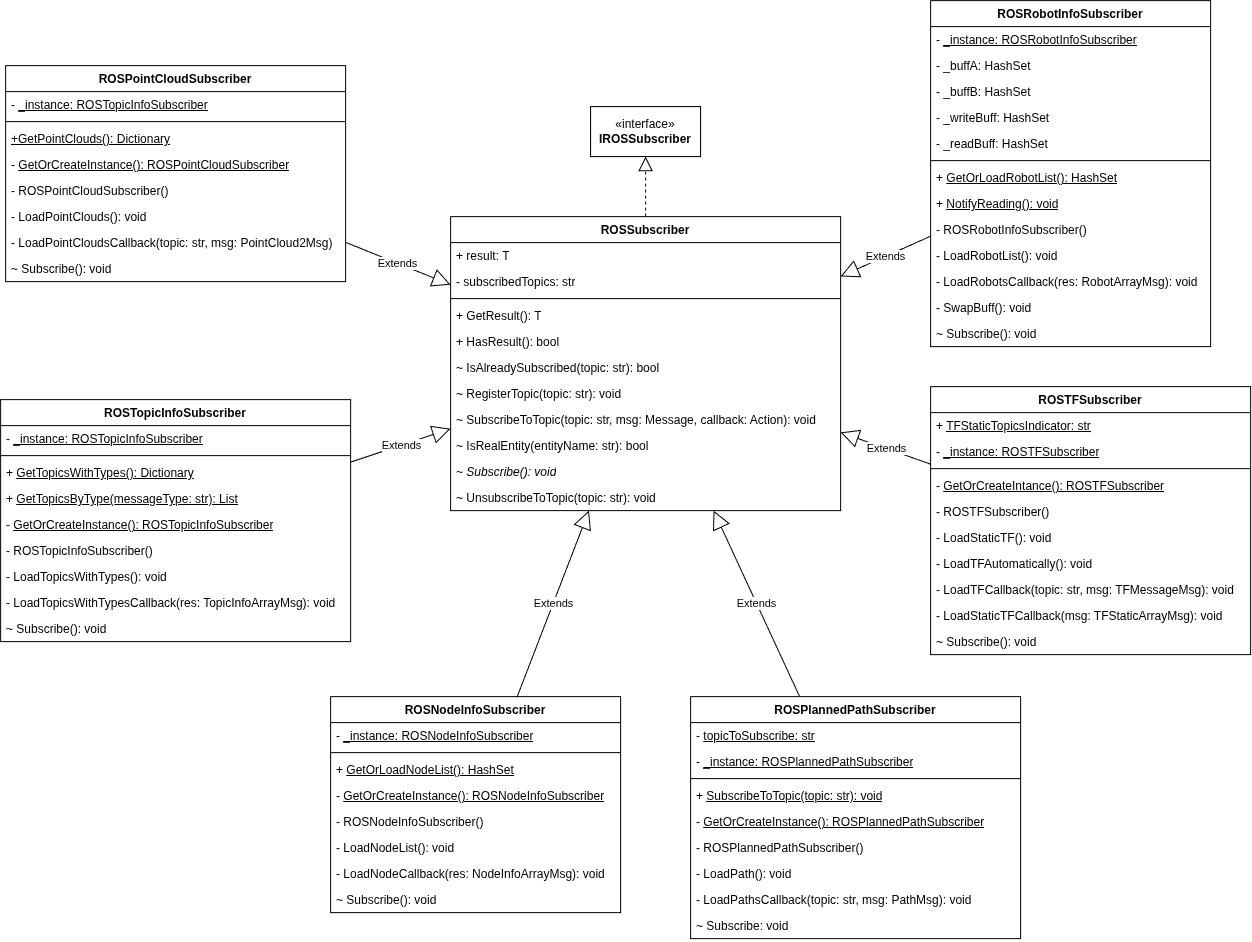
\includegraphics[width=0.8\textwidth]{imagenes/diagramas/ROSSubscriber.png}
    \caption{Módulo ROSSubscriber}
    \label{fig:ros_subscriber_module}
\end{figure}

De forma similar al módulo de suscripción a temas, el módulo de publicación de temas de ROS se muestra 
en la Figura \ref{fig:ros_service_module}.
Este es el encargado de gestionar la comunicación con los servicios publicados en los nodos, para ello, 
se emplea la clase base \textit{ROSService} que permite la invocación de cualquier servicio de ROS.
\begin{figure}[htbp]
    \centering
    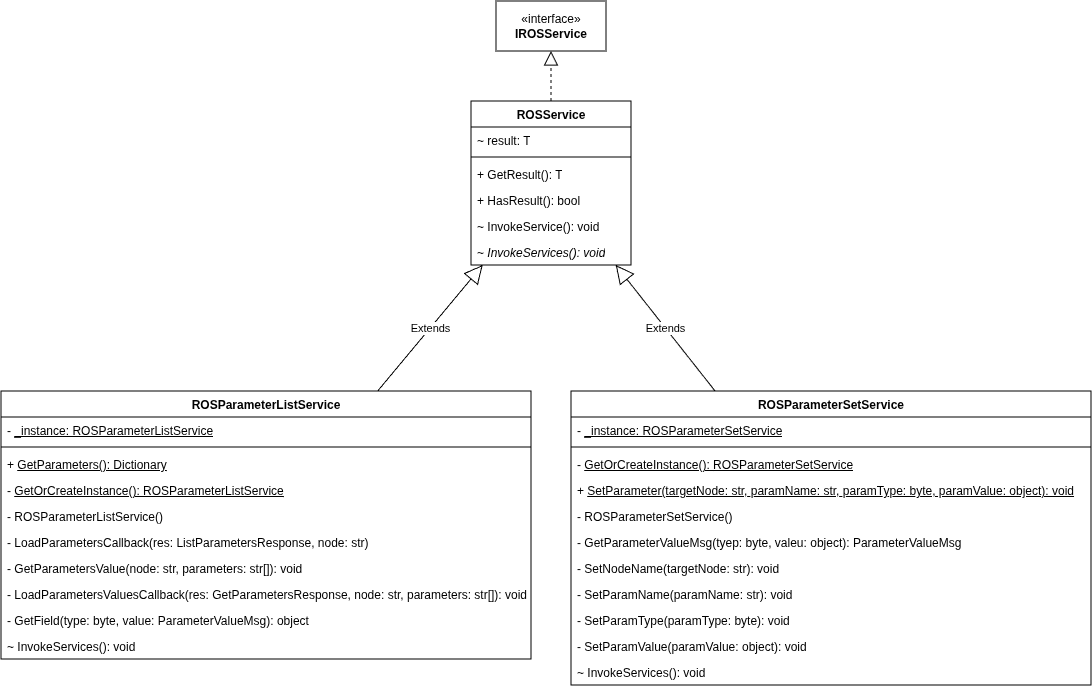
\includegraphics[width=0.8\textwidth]{imagenes/diagramas/ROSService.png}
    \caption{Módulo ROSService}
    \label{fig:ros_service_module}
\end{figure}


\section{Implementación del sistema}
La aplicación está dividida en diferentes módulos con diversas interdependencias. 
Entre ellos destacan principalemente el de detección de \textit{AprilTags}, es decir, 
el sistema de detección de puntos de referencia, la visualización de las transformaciones 
-- y sus consecuentes datos como velocidad angular y lineal, posición, rotación, \textit{jitter}, etc. -- y 
el control y visualización espacial de los robots.

En cuanto al primer módulo, se trata de la librería \textbf{AprilRobotics/apriltag} desarrollada en C compilada como 
dependenicia externa para ser empleada como \textit{plugin} en Unity. Cada \textit{frame} de la camara de la aplicación se transforma 
a escala de grises, se invierte para acomodarse a los requisitos de la aplicación y se envía al \textit{plugin} donde se identifican 
las etiquetas presentes en la imagen. Esta dependencia devuelve la estructura de datos con la información necesaria de las etiquetas
-- en este caso: el identificador y la posición con respecto a la imagen --, de forma que si una etiqueta es nueva en el sistema 
(no ha sido almacenada en la base de datos de etiquetas), se interpela al usuario para que realice la asociación con el \textit{frame} de las
transformaciones de ROS y el \textit{topic} empleado en la visualización del camino proyectado correspondiente. Este módulo puede considerarse,
junto al de la visualización de las transformaciones, como el núcleo principal de la aplicación, puesto que es el encargado de hacer 
converger el mundo virtual con el físico.

La visualización de las transformaciones de ROS se lleva a cabo en el módulo \textbf{TF}. Este se encarga  reconstruir la jerarquía de ROS en Unity 
procesando los mensajes que los nodos publican en los \textit{topics} de transformación -- aquellos que contienen mensajes del tipo \textit{TFMessage} --
y creando los objetos de juego (\textit{GameObjects}) que permitirán visualizar diferentes datos como las orientaciones de un brazo robótico, la velocidad
lineal de un robot móvil o su velocidad angular y problemas característicos en la robótica como el \textit{jitter}, los saltos, el \textit{trail}, \textit{flipping}, etc.
Es el módulo que permite conocer el estado del sistema en todo momento, lo que da el sentido al resto de funcionalidades de la aplicación.

La visualización espacial puede considerarse una complementación al módulo anterior, puesto que es el encargado de situar en el mundo mediante la realidad aumentada 
el estado de los sensores de detección de profundidad como \textit{LiDAR}. Este se trata de un módulo de inicialización activa, es decir, en el caso de que el robot cuente 
con un sensor que emita mensajes \textit{PointCloud2}, el usuario debe asociar al \textit{frame} correspondiente el \textit{topic} donde se publiquen dichos mensajes.
Se estudió la manera de realizar este emparejamiento de forma automática, pero debido a que el usuario final puede no seguir una convención concreta de nombres
en los \textit{topics}, es preferible que sea este quien realice la confirmación de la información; de otra manera, la información que se muestre puede ser errónea y 
eventualmente propiciar accidentes.

El control espacial permite que robots móviles puedan ser operados empleando la aplicación mediante control directo (teleoperación) o planificación de ruta (\textit{path planning}).
La operación telemática esta compuesta por un sistema multimodal que permite, mediante el accionamiento de un \textit{joystick} y botones virtuales, el control total
de un robot concreto.
La planificación de ruta, a su vez, permite situar de forma virtual marcas en las superficies interactuables en realidad aumentada -- aquellas captadas por las cámaras y 
trasformadas en planos dentro del mundo digital -- que posteriormente son transformadas en localizaciones del mundo real a las que los robots móviles acudirán cumpliendo la ruta 
programada. Puesto que ejecutar la acción del movimiento cuando el usuario posiciona una marca de referencia no es seguro ni práctico ni sigue la filosofía de la planificación, 
el usuario será quien decida cuando ejecutar cada plan en cada robot.

Además de los mencionados anteriormente, existen submódulos que proporcionan funcionalidades que los usuarios pueden considerar como de gran importancia para 
la consecución de sus objetivos con la aplicación. Entre ellos destacan los módulos de publicación y observación de mensajes en \textit{topics}. Con estas funcionalidades
pueden realizarse acciones en robots que no tienen actualmente una función específica desarrollada en la aplicación o suscribirse a cadenas de mensajes en un robot para observar
qué es lo que le ocurre en caso de problemas no descubiertos.

\section{Validación y pruebas}

\subsection{Pruebas del CU-01: Configuración conexión ROS}
\begin{longtable}{|p{1.5cm}|p{4cm}|p{4cm}|}
\hline
\textbf{ID} & \textbf{Datos de entrada} & \textbf{Resultado esperado} \\
\hline
CP-01 & IP y puerto válidos & Conexión establecida \\
\hline
CP-02 & IP incorrecta & Mensaje de error \\
\hline
CP-03 & Puerto incorrecto & Mensaje de error \\
\hline
CP-04 & Campos vacíos & Validación de campos obligatorios \\
\hline
\caption{Casos de prueba de la configuración de conexión con ROS}
\end{longtable}

\subsection{Pruebas del CU-02: Configuración idioma}
\begin{longtable}{|p{1.5cm}|p{4cm}|p{4cm}|}
\hline
\textbf{ID} & \textbf{Datos de entrada} & \textbf{Resultado esperado} \\
\hline
CP-05 & Castellano seleccionado & Cambio textos aplicación a español \\
\hline
CP-06 & Inglés seleccionado & Cambio textos aplicación a inglés \\
\hline
\caption{Casos de prueba de la configuración de idioma}
\end{longtable}

\subsection{Pruebas del CU-03: Asignación de \textit{frame} a \textit{AprilTag}}
\begin{longtable}{|p{1.5cm}|p{4cm}|p{4cm}|}
\hline
\textbf{ID} & \textbf{Datos de entrada} & \textbf{Resultado esperado} \\
\hline
CP-07 & \textit{Frame} seleccionado & Asociación \textit{AprilTag}-\textit{frame} establecida \\
\hline
\caption{Casos de prueba de la asignación de \textit{frame} a \textit{AprilTag}}
\end{longtable}

\subsection{Pruebas del CU-04: Configuración de nube de puntos}
\begin{longtable}{|p{1.5cm}|p{4cm}|p{4cm}|}
\hline
\textbf{ID} & \textbf{Datos de entrada} & \textbf{Resultado esperado} \\
\hline
CP-08 & Selección \textit{topic} para un \textit{frame} & Asociación \textit{frame}-\textit{topic} de nube de puntos establecida (visualización de la nube de puntos en el \textit{frame})\\
\hline
\caption{Casos de prueba de la configuración de nube de puntos}
\end{longtable}

\subsection{Pruebas del CU-05: Configuración visualización ruta planificada}
\begin{longtable}{|p{1.5cm}|p{4cm}|p{4cm}|}
\hline
\textbf{ID} & \textbf{Datos de entrada} & \textbf{Resultado esperado} \\
\hline
CP-09 & Selección \textit{topic} para el \textit{AprilTag} & Asociación \textit{AprilTag}-\textit{topic} de ruta planificada establecida (visualización de la ruta en caso de existir) \\
\hline
\caption{Casos de prueba de configuración de visualización de ruta planificada}
\end{longtable}

\subsection{Pruebas del CU-06: Visualizar/Ocultar \textit{frames}}
\begin{longtable}{|p{1.5cm}|p{4cm}|p{4cm}|}
\hline
\textbf{ID} & \textbf{Datos de entrada} & \textbf{Resultado esperado} \\
\hline
CP-10 & Selección ocultación \textit{frame} & \textit{Frame} deja de visualizarse al usuario \\
\hline
CP-11 & Selección visualización \textit{frame} & \textit{Frame} se visualiza al usuario \\
\hline
\caption{Casos de prueba de visualización/ocultación de \textit{frames}}
\end{longtable}

\subsection{Pruebas del CU-07: Teleoperación}
\begin{longtable}{|p{1.5cm}|p{4cm}|p{4cm}|}
\hline
\textbf{ID} & \textbf{Datos de entrada} & \textbf{Resultado esperado} \\
\hline
CP-12 & Mensaje de avance & Robot se mueve a velocidad lineal establecida hacia adelante \\
\hline
CP-13 & Mensaje de retroceso & Robot se mueve a velocidad lineal establecida hacia atrás \\
\hline
CP-14 & Mensaje de giro hacia izquierda & Robot se gira a velocidad angular establecida hacia izquierda \\
\hline
CP-15 & Mensaje de giro hacia derecha & Robot se gira a velocidad angular establecida hacia derecha \\
\hline
CP-16 & Mensaje de subida & Robot sube el elemento correspondiente a velocidad establecida \\
\hline
CP-17 & Mensaje de bajada & Robot baja el elemento correspondiente a velocidad establecida \\
\hline
\caption{Casos de prueba de teleoperación}
\end{longtable}

\subsection{Pruebas del CU-08: Planificar ruta}
\begin{longtable}{|p{1.5cm}|p{4cm}|p{4cm}|}
\hline
\textbf{ID} & \textbf{Datos de entrada} & \textbf{Resultado esperado} \\
\hline
CP-18 & Posición de marca de referencia añadida & La marca se visualiza encadenada a la anterior (o al robot en caso de ser la primera) en la posición establecida \\
\hline
CP-19 & Accionamiento de eliminación de marca de referencia & La ultima marca se deja de visualizar \\
\hline
CP-20 & Mensaje de la ruta planificada & Robot se desplaza consecutivamente a todos los puntos de la ruta \\
\hline
\caption{Casos de prueba de planificación de ruta}
\end{longtable}

\subsection{Pruebas del CU-09: Medición entre \textit{frames}}
\begin{longtable}{|p{1.5cm}|p{4cm}|p{4cm}|}
\hline
\textbf{ID} & \textbf{Datos de entrada} & \textbf{Resultado esperado} \\
\hline
CP-21 & Selección primer \textit{frame} & \textit{Frame} se visualiza en otro color y textura \\
\hline
CP-22 & Selección segundo \textit{frame} & \textit{Frame} se visualiza en otro color y textura y se muestra la distancia, giro, etc. entre ellos \\
\hline
\caption{Casos de prueba de medición entre \textit{frames}}
\end{longtable}

\subsection{Pruebas del CU-10: Ajuste de posición de \textit{frames} asignados a marcas visuales}
\begin{longtable}{|p{1.5cm}|p{4cm}|p{4cm}|}
\hline
\textbf{ID} & \textbf{Datos de entrada} & \textbf{Resultado esperado} \\
\hline
CP-23 & Selección \textit{frame} & \textit{Frame} se visualiza en otro color y textura \\
\hline
CP-24 & Mensaje de desplazamiento a izquierda & \textit{Frame} junto con hijos se desplazan hacia la izquierda \\
\hline
CP-25 & Mensaje de desplazamiento a derecha & \textit{Frame} junto con hijos se desplazan hacia la derecha \\
\hline
CP-26 & Mensaje de desplazamiento hacia delante & \textit{Frame} junto con hijos se desplazan hacia delante \\
\hline
CP-27 & Mensaje de desplazamiento hacia atrás & \textit{Frame} junto con hijos se desplazan hacia atrás \\
\hline
CP-28 & Mensaje de desplazamiento hacia arriba & \textit{Frame} junto con hijos se desplazan hacia arriba \\
\hline
CP-29 & Mensaje de desplazamiento hacia abajo & \textit{Frame} junto con hijos se desplazan hacia abajo \\
\hline
\caption{Casos de prueba del ajuste de la posición de \textit{frames} asigandos a marcas visuales}
\end{longtable}

\subsection{Pruebas del CU-11: Ajuste de escala de \textit{frames} asignados a marcas visuales}
\begin{longtable}{|p{1.5cm}|p{4cm}|p{4cm}|}
\hline
\textbf{ID} & \textbf{Datos de entrada} & \textbf{Resultado esperado} \\
\hline
CP-30 & Selección \textit{frame} & \textit{Frame} se visualiza en otro color y textura \\
\hline
CP-31 & Aumento de escala & \textit{Frame} se visualiza más grande \\
\hline
CP-32 & Disminución de escala & \textit{Frame} se visualiza más pequeño \\
\hline
\caption{Casos de prueba del ajuste de escala de \textit{frames} asignados a marcas visuales}
\end{longtable}

\subsection{Pruebas del CU-12: Suscripción a \textit{topics}}
\begin{longtable}{|p{1.5cm}|p{4cm}|p{4cm}|}
\hline
\textbf{ID} & \textbf{Datos de entrada} & \textbf{Resultado esperado} \\
\hline
CP-33 & Selección \textit{topic} & Se visualizan los mensajes publicados por los nodos en el \textit{topic} \\
\hline
\caption{Casos de prueba de la suscripción a \textit{topics}}
\end{longtable}

\subsection{Pruebas del CU-13: Publicación en \textit{topics}}
\begin{longtable}{|p{1.5cm}|p{4cm}|p{4cm}|}
\hline
\textbf{ID} & \textbf{Datos de entrada} & \textbf{Resultado esperado} \\
\hline
CP-34 & Mensaje mal formulado & Se muestra mensaje de error \\
\hline
CP-35 & Frecuencia errónea & El sistema corrige la entrada de usuario estableciendo un valor válido \\
\hline
\caption{Casos de prueba de la publicación en \textit{topics}}
\end{longtable}

\subsection{Pruebas del CU-14: Modificación de parámetros en nodos}
\begin{longtable}{|p{1.5cm}|p{4cm}|p{4cm}|}
\hline
\textbf{ID} & \textbf{Datos de entrada} & \textbf{Resultado esperado} \\
\hline
CP-36 & Valor erróneo de parámetro & Se muestra mensaje de error \\
\hline
\caption{Casos de prueba de la modificación de parámetros}
\end{longtable}

\section{Consideraciones éticas y legales}
Todas las etapas de desarrollo del proyecto han sido enfocadas considerando a los usuarios como el núcleo central de la usabilidad dentro de la aplicación, 
teniendo en cuenta de forma primordial la reducción de la carga cognitiva necesaria para la toma de decisiones, a la par que se intenta salvaguardar sus 
intereses, integridad física y psicológica. Así pues, se prima la simplificación en los procesos repetitivos y tediosos como la navegación excesiva por menús, optando 
por elementos interactuables sencillos y visuales; sin embargo, se evita realizar suposiciones ante situaciones que puedan conllevar un riesgo hacia la integridad 
del usuario, por ello la aplicación cuenta con diferentes configuraciones en las que se solicita la verificación de los datos.

En cuanto al licenciamiento \textit{software}, se ha optado por incluir dependencias de las que se pueda comprobar su trazabilidad sin impedimento, de manera que 
cualquier desarrollador o persona con conocimientos de programación pueda verificar la integridad e intencionalidad de los algoritmos utilizados. Por ello, durante
el desarrollo del proyecto se emplearán librerías \textit{opensource} con licencias \textit{MIT}, \textit{BSD} y \textit{Apache2} entre otras.

El resultado final, de igual forma, deberá poder ser trazado libremente y emplearse en contextos de forma que se salvaguarden las condiciones de uso de sus dependencias. 
Contará, de esta manera, con una licencia no más restrictiva que las dependencias que lo componen.

Cabe destacar, por otro lado, que algunos iconos de la aplicación han sido generados empleando inteligencia artificial generativa al ser imágenes sencillas y reproducibles 
fácilmente por un ser humano.